% !TEX TS-program = pdflatex
% !TEX encoding = UTF-8 Unicode

% This is a simple template for a LaTeX document using the "article" class.
% See "book", "report", "letter" for other types of document.

\documentclass[11pt]{article} % use larger type; default would be 10pt

\usepackage[utf8]{inputenc} % set input encoding (not needed with XeLaTeX)

%%% Examples of Article customizations
% These packages are optional, depending whether you want the features they provide.
% See the LaTeX Companion or other references for full information.

%%% PAGE DIMENSIONS
\usepackage{geometry} % to change the page dimensions
\geometry{letterpaper} % or letterpaper (US) or a5paper or....
% \geometry{margin=2in} % for example, change the margins to 2 inches all round
% \geometry{landscape} % set up the page for landscape
%   read geometry.pdf for detailed page layout information

\usepackage{graphicx} % support the \includegraphics command and options
\graphicspath{ {./images/} }

% \usepackage[parfill]{parskip} % Activate to begin paragraphs with an empty line rather than an indent

%%% PACKAGES
\usepackage{booktabs} % for much better looking tables
\usepackage{array} % for better arrays (eg matrices) in maths
\usepackage{paralist} % very flexible & customisable lists (eg. enumerate/itemize, etc.)
\usepackage{verbatim} % adds environment for commenting out blocks of text & for better verbatim
\usepackage{subcaption} % make it possible to include more than one captioned figure/table in a single float
% These packages are all incorporated in the memoir class to one degree or another...

\usepackage{siunitx}
\usepackage{hyperref}
\usepackage[table]{xcolor}

%%% HEADERS & FOOTERS
\usepackage{fancyhdr} % This should be set AFTER setting up the page geometry
\pagestyle{fancy} % options: empty , plain , fancy
\renewcommand{\headrulewidth}{0pt} % customise the layout...
\lhead{}\chead{}\rhead{}
\lfoot{}\cfoot{\thepage}\rfoot{}

%%% SECTION TITLE APPEARANCE
\usepackage{sectsty}
\allsectionsfont{\sffamily\mdseries\upshape} % (See the fntguide.pdf for font help)
% (This matches ConTeXt defaults)

%%% ToC (table of contents) APPEARANCE
\usepackage[nottoc,notlof,notlot]{tocbibind} % Put the bibliography in the ToC
\usepackage[titles,subfigure]{tocloft} % Alter the style of the Table of Contents
\renewcommand{\cftsecfont}{\rmfamily\mdseries\upshape}
\renewcommand{\cftsecpagefont}{\rmfamily\mdseries\upshape} % No bold!

%%% END Article customizations

%%% The "real" document content comes below...

\title{Combining Motor, Speed, and Phase PID responses}
\author{Andy Berger}
%\date{} % Activate to display a given date or no date (if empty),
         % otherwise the current date is printed 

\begin{document}
\maketitle

\section{Combined Speed and Phase PID}
The following assumes PID controllers of the form:
\begin{equation}
\mathrm{Output} = P \mathcal{E}_i + I \sum_{k=0}^i \mathcal{E}_k \Delta t + D \frac{(\mathcal{E}_i - \mathcal{E}_{i-1})}{\Delta t}
\end{equation}

\noindent where $\mathcal{E}_i$ is the $i^{th}$ error signal measurement, defined as (Setpoint - Measured Value).

Presently, the SR542 chopper head is controlled by a PID controller of the motor's phase, and a PI controller of it's speed. For a PID controller of motor phase (in the Laplace, or s-domain), with proportional, integral, and derivative gains $P_{\theta}$, $I_{\theta}$, and $D_{\theta}$ respectively:
\begin{equation}
I_Q = \left(P_{\theta} + \frac{I_{\theta}}{s}  + D_{\theta}s\right) (\theta_\mathrm{ref} - \theta)
\end{equation}

\noindent And for a PI controller of speed:
\begin{eqnarray}
I_Q &=& \left(P_{\omega} + \frac{I_{\omega}}{s}\right) (\omega_\mathrm{ref} - \omega) \nonumber \\
&=& \left(P_{\omega} + \frac{I_{\omega}}{s}\right) (\theta_\mathrm{ref} s - \theta s) \nonumber \\
&=& \left(P_{\omega} s + I_{\omega}\right) (\theta_\mathrm{ref} - \theta)
\end{eqnarray}

\noindent So that the total PID-controlled current $I_Q$ is given by, grouping terms of the same order of $s$
\begin{equation}
I_Q = \left[(P_{\theta} + I_{\omega}) + \frac{I_{\theta}}{s}  + (D_{\theta} + P_{\omega})s\right] (\theta_\mathrm{ref} - \theta) 
\label{eq:totalPID}
\end{equation}

\noindent From Eq. \ref{eq:totalPID} it is plain to see that with regards to the dynamics of $\theta$, $I_\omega$ acts as an effective proportional gain and $P_\omega$ acts as a derivative gain. Therefore, to apply the Ziegler-Nichols technique for closed-loop tuning, in which case it is necessary to begin with $I$ and $D = 0$, we must set $P_\omega = 0$, and include $I_\omega$ when determining $K_u$, the so-called ``ultimate'' proportional gain that causes sustained oscillations of $\theta$.

\subsection{Closed-Loop Ziegler-Nichols Tuning}

From the SIM960 Manual, we can use Zeigler-Nichols closed-loop tuning method:
\begin{enumerate}
\item Set $P_\theta$, $I_\theta$, and $P_\theta = 0$ (disabled phase PID)
\item Allow speed PID to bring motor up to speed
\item Set $P_\omega = 0$, since this acts as an effective derivative gain with regards to phase $\theta$. The motor should maintain speed stability
\item Start to increase $P_\theta$ until oscillations of phase remain consistent (not decaying away. Also, further increase of $P_\theta$ should cause increasing oscillation). This value of $P_\theta$ is recorded as $K_u$, the ``ultimate gain'' needed for undamped (neither overdamped nor underdamped) oscillations of the phase.  amplitude. 
\item Record the period of oscillations as $T_u$.
\end{enumerate}

\noindent The values $K_u$ and $T_u$ are then used to determined the PID gains for a critically damped response of the phase to a step change in the phase setpoint using the formulae in Table \ref{tab:ZieglerNichols}. I found that undamped oscillations occured at $P_\theta = 1.5$, with an oscillation period of $T_u = 0.523$ sec. Therefore $K_u = P_\phi + I_\omega = 1.5184$ ($I_\omega$ was previously determined using Ziegler-Nichols open-loop tuning by measuring the impulse response of the motor speed $\omega$. See Table \ref{tab:MotorParams}).
\begin{table}[h]
\centering
\begin{tabular}{ r | l | l }
\hline
\textbf{Parameter} & \textbf{Formula} & \textbf{Value}  \\
\hline
$P$ & $3 K_u/5$ & 0.911\\
$I$ & $P*2/T_u$ & 3.484\\
$D$ & $P*T_u/8$ & 0.060
\end{tabular}
\caption{P, I, and D gains for a PID controller, as determined by the ultimate gain $K_u$ and the oscillation period $T_u$.}
\label{tab:ZieglerNichols}
\end{table}

\noindent Empirically, the values determined in Table \ref{tab:ZieglerNichols} are substantially different---and more importantly, do not work better---than the best-case parameters determined empirically (and listed in Table \ref{tab:MotorParams}). \textbf{I haven't figured out why the Ziegler-Nichols method fails}.

\section{Closed Loop Response Function}
Starting from Newton's Second Law, we sum the torques acting on the motor:
\begin{equation}
J \ddot{\theta} + \Gamma \dot{\theta} = K_T I_Q
\label{eq:Newton2}
\end{equation}

\noindent where $\theta$ is the motor rotation angle, $K_T$ is the torque constant (in \si{N.m/A}), $J$ is the moment of inertia (in \si{kg.m^2}), $\Gamma$ is the damping constant (in \si{N.m.s}), and $I_Q$ is the current applied to the Q-axis (in the D-Q reference frame, the Q-axis is responsible for the torque applied to the rotor moment). This quantity is controlled by the combined PID control, as derived in Eq. \ref{eq:totalPID}.

Combining Eqs. \ref{eq:totalPID} and \ref{eq:Newton2}, we find:
\begin{equation}
J s^2 \theta + \Gamma s \theta = K_T \left[(P_{\theta} + I_{\omega}) + \frac{I_{\theta}}{s}  + (D_{\theta} + P_{\omega})s\right] (\theta_\mathrm{ref} - \theta) 
\label{eq:Newton2withPID}
\end{equation}

\noindent Define $G_\mathrm{motor} \equiv  K_T/(J s^2 \theta + \Gamma s)$ and $G_\mathrm{PID} \equiv ((P_{\theta} + I_{\omega}) + I_{\theta}/s  + (D_{\theta} + P_{\omega})s)$, then the response function of motor phase $\theta$ is given by:

\begin{equation}
\theta(s) = \left[\frac{G_\mathrm{motor} G_\mathrm{PID}}{1 + G_\mathrm{motor} G_\mathrm{PID}}\right] \theta_\mathrm{ref}(s)
\end{equation}

The motor response parameters are determined from impulse response measurements\footnote{$\Gamma$ is actually a function of frequency, unlike in the constant damping model assumed here. Depending on the speed, I have found that $\Gamma \propto K_{D,0} \omega^x$, where $x$ ranges from 0 to 0.8, such that the torque term scales as $\omega^{1+x}$. For simplicity, I assume $x=1$.}. The PID gains are determined using Ziegler-Nichols open-loop tuning (for $P_\omega$ and $I_\omega$) or empirically (for phase PID gains).

\begin{table}
\centering
\begin{tabular}{| l | l | l |}
\hline
\textbf{Parameter} & \textbf{Value} & \textbf{Source} \\
\hline
$K_T$ & \SI{5.55}{mN.m/A} & Nuelectronics 16-mm brushless motor spec sheet \\
$J$ & \SI{1.82e-5}{kg.m^2} & Accel. vs $I_Q$ \\
$K_{D,0}$ & \SI{1.42e-8}{} & $I_Q$ vs. $\omega_\mathrm{term}$ \\
$\Gamma$ & $K_{D,0} \omega_\mathrm{final}$ & approximation needed for single-valued $\Gamma$ \\
\hline
$P_\theta$ & 0.5 & empirical tuning \\
$I_\theta$ & 0.5 & empirical tuning \\
$D_\theta$ & 0.1 to 5 & empirical tuning, depending on phase-lock status \\
\hline
$P_\omega$ & 0.0231 & Ziegler-Nichols \\
$I_\omega$ & 0.0184 & Ziegler-Nichols \\
\hline
\end{tabular}
\caption{Motor parameters extracted from impulse response tests, and PID gains as determined by Ziegler-Nichols methods, or empirically}
\label{tab:MotorParams}
\end{table}

Using the values from Table \ref{tab:MotorParams}, the Bode and Step Response of the closed loop system can be calculated numerically (using Python's scipy.signal module). Fig. \ref{fig:Bode} was enlightening, as I previous observed large, slow oscillations in the controlled phase (at 1-2 Hz) when $D_\theta = 0.1$. I believe this is due to the gain peaking seen at low frequencies (even though there isn't exact numerical agreement between the oscillation frequency and the location of the gain peaking, which occurs at $\sim$0.6 Hz. Nevertheless, the $D_\theta = 5$ response eliminates that gain peaking and experimentally, the phase oscillations vanish for that choice of derivative gain, such that at least the qualitative behavior can be understood in light of Fig. \ref{fig:Bode}. Furthermore, the Bode analysis shows that the PID gains determined by the Ziegler-Nichols technique can be expected to perform very poorly, as the gain peaking is most substantial here.

\begin{figure}
\centering
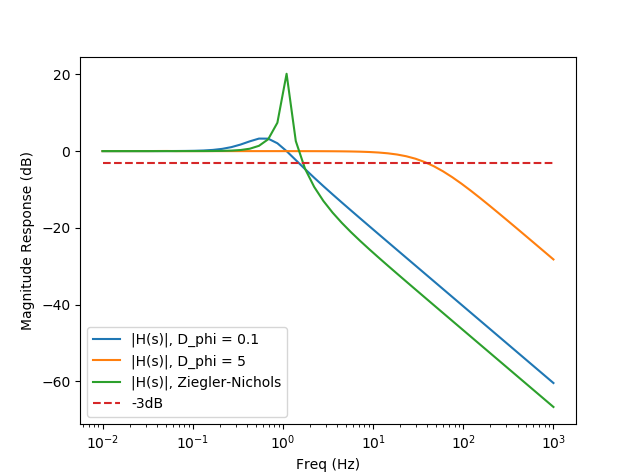
\includegraphics[scale=0.75]{ClosedLoopBodePlot.png}
\caption{Bode plot of motor + phase and speed PID response, showing the effect of $D_\theta$}
\label{fig:Bode}
\end{figure}

\begin{figure}
\centering
	\begin{subfigure}[t]{0.5\textwidth}
		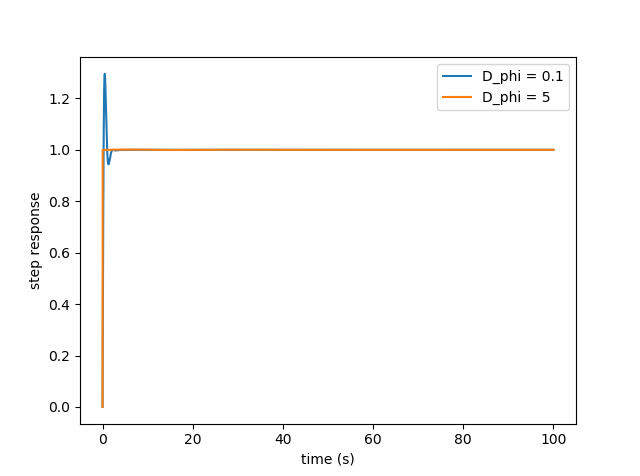
\includegraphics[width=\linewidth]{StepResponse.png}
		\caption{}
		\label{fig:StepResponse}
	\end{subfigure}%
	\begin{subfigure}[t]{0.5\textwidth}
		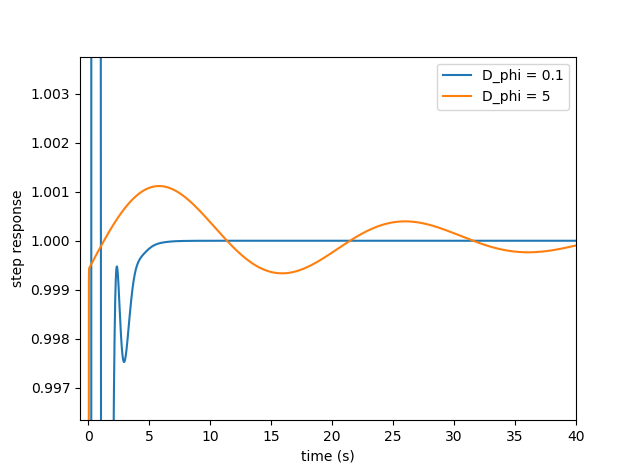
\includegraphics[width=\linewidth]{StepResponse_zoom.png}
		\caption{Same as \ref{fig:StepResponse}, but zoomed on short time scales}
		\label{fig:StepResponse_zoom}
	\end{subfigure}
	\caption{Step response of motor + phase and speed PID response, showing the effect of $D_\theta$. \textbf{I don't totally trust these simulation results due to the discontinuity of the derivative in the $D_\theta = 5$ response at short time scales}.}
\end{figure}


\end{document}
